% Created by tikzDevice version 0.8.1 on 2015-11-17 12:44:46
% !TEX encoding = UTF-8 Unicode
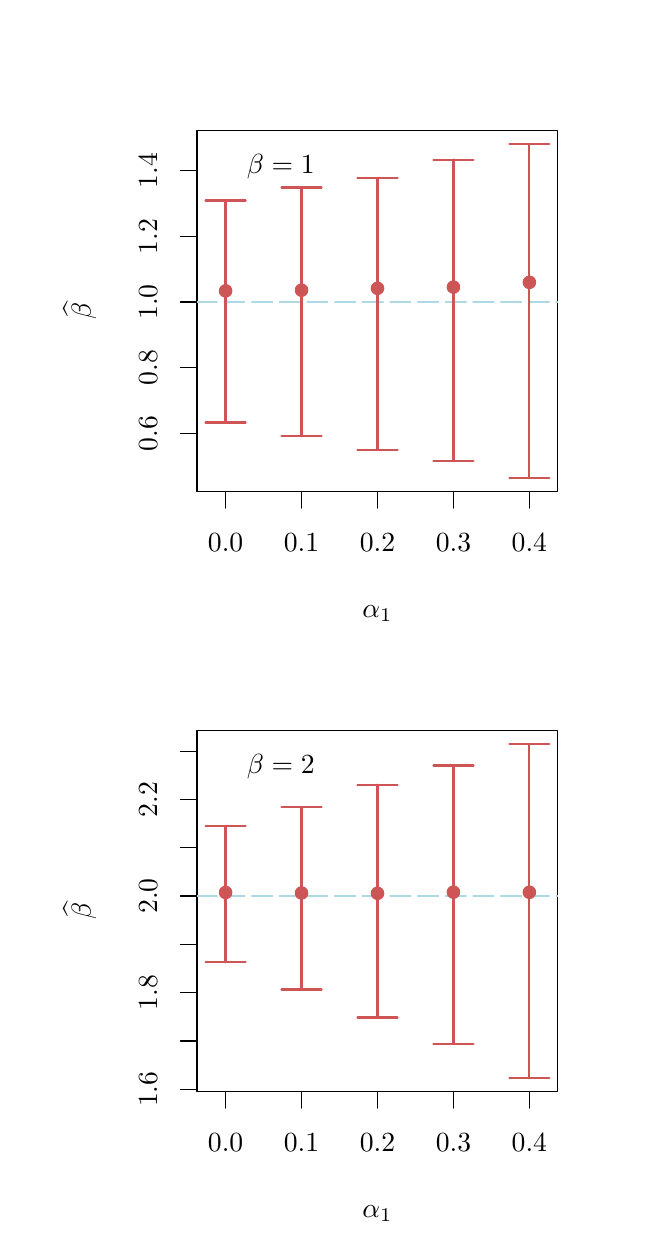
\begin{tikzpicture}[x=1pt,y=1pt]
\definecolor{fillColor}{RGB}{255,255,255}
\path[use as bounding box,fill=fillColor,fill opacity=0.00] (0,0) rectangle (216.81,433.62);
\begin{scope}
\path[clip] ( 61.20,266.01) rectangle (191.61,396.42);
\definecolor{drawColor}{RGB}{255,255,255}
\definecolor{fillColor}{RGB}{255,255,255}

\path[draw=drawColor,line width= 0.4pt,line join=round,line cap=round,fill=fillColor] ( 71.52,338.50) circle (  2.25);

\path[draw=drawColor,line width= 0.4pt,line join=round,line cap=round,fill=fillColor] ( 98.96,338.76) circle (  2.25);

\path[draw=drawColor,line width= 0.4pt,line join=round,line cap=round,fill=fillColor] (126.41,339.43) circle (  2.25);

\path[draw=drawColor,line width= 0.4pt,line join=round,line cap=round,fill=fillColor] (153.85,339.87) circle (  2.25);

\path[draw=drawColor,line width= 0.4pt,line join=round,line cap=round,fill=fillColor] (181.29,341.59) circle (  2.25);
\end{scope}
\begin{scope}
\path[clip] (  0.00,  0.00) rectangle (216.81,433.62);
\definecolor{drawColor}{RGB}{0,0,0}

\path[draw=drawColor,line width= 0.4pt,line join=round,line cap=round] ( 71.52,266.01) -- (181.29,266.01);

\path[draw=drawColor,line width= 0.4pt,line join=round,line cap=round] ( 71.52,266.01) -- ( 71.52,260.01);

\path[draw=drawColor,line width= 0.4pt,line join=round,line cap=round] ( 98.96,266.01) -- ( 98.96,260.01);

\path[draw=drawColor,line width= 0.4pt,line join=round,line cap=round] (126.41,266.01) -- (126.41,260.01);

\path[draw=drawColor,line width= 0.4pt,line join=round,line cap=round] (153.85,266.01) -- (153.85,260.01);

\path[draw=drawColor,line width= 0.4pt,line join=round,line cap=round] (181.29,266.01) -- (181.29,260.01);

\node[text=drawColor,anchor=base,inner sep=0pt, outer sep=0pt, scale=  1.00] at ( 71.52,244.41) {0.0};

\node[text=drawColor,anchor=base,inner sep=0pt, outer sep=0pt, scale=  1.00] at ( 98.96,244.41) {0.1};

\node[text=drawColor,anchor=base,inner sep=0pt, outer sep=0pt, scale=  1.00] at (126.41,244.41) {0.2};

\node[text=drawColor,anchor=base,inner sep=0pt, outer sep=0pt, scale=  1.00] at (153.85,244.41) {0.3};

\node[text=drawColor,anchor=base,inner sep=0pt, outer sep=0pt, scale=  1.00] at (181.29,244.41) {0.4};

\path[draw=drawColor,line width= 0.4pt,line join=round,line cap=round] ( 61.20,287.03) -- ( 61.20,381.92);

\path[draw=drawColor,line width= 0.4pt,line join=round,line cap=round] ( 61.20,287.03) -- ( 55.20,287.03);

\path[draw=drawColor,line width= 0.4pt,line join=round,line cap=round] ( 61.20,310.75) -- ( 55.20,310.75);

\path[draw=drawColor,line width= 0.4pt,line join=round,line cap=round] ( 61.20,334.48) -- ( 55.20,334.48);

\path[draw=drawColor,line width= 0.4pt,line join=round,line cap=round] ( 61.20,358.20) -- ( 55.20,358.20);

\path[draw=drawColor,line width= 0.4pt,line join=round,line cap=round] ( 61.20,381.92) -- ( 55.20,381.92);

\node[text=drawColor,rotate= 90.00,anchor=base,inner sep=0pt, outer sep=0pt, scale=  1.00] at ( 46.80,287.03) {0.6};

\node[text=drawColor,rotate= 90.00,anchor=base,inner sep=0pt, outer sep=0pt, scale=  1.00] at ( 46.80,310.75) {0.8};

\node[text=drawColor,rotate= 90.00,anchor=base,inner sep=0pt, outer sep=0pt, scale=  1.00] at ( 46.80,334.48) {1.0};

\node[text=drawColor,rotate= 90.00,anchor=base,inner sep=0pt, outer sep=0pt, scale=  1.00] at ( 46.80,358.20) {1.2};

\node[text=drawColor,rotate= 90.00,anchor=base,inner sep=0pt, outer sep=0pt, scale=  1.00] at ( 46.80,381.92) {1.4};

\path[draw=drawColor,line width= 0.4pt,line join=round,line cap=round] ( 61.20,266.01) --
	(191.61,266.01) --
	(191.61,396.42) --
	( 61.20,396.42) --
	( 61.20,266.01);
\end{scope}
\begin{scope}
\path[clip] (  0.00,216.81) rectangle (216.81,433.62);
\definecolor{drawColor}{RGB}{0,0,0}

\node[text=drawColor,anchor=base,inner sep=0pt, outer sep=0pt, scale=  1.00] at (126.41,220.41) {$\alpha_1$};

\node[text=drawColor,rotate= 90.00,anchor=base,inner sep=0pt, outer sep=0pt, scale=  1.00] at ( 22.80,331.22) {$\widehat{\beta}$};
\end{scope}
\begin{scope}
\path[clip] ( 61.20,266.01) rectangle (191.61,396.42);
\definecolor{drawColor}{RGB}{0,0,0}

\node[text=drawColor,anchor=base west,inner sep=0pt, outer sep=0pt, scale=  1.00] at ( 79.20,380.98) {$\beta=1$};
\definecolor{drawColor}{RGB}{173,216,230}

\path[draw=drawColor,line width= 0.8pt,dash pattern=on 7pt off 3pt ,line join=round,line cap=round] ( 61.20,334.48) -- (191.61,334.48);

\path[draw=drawColor,line width= 0.8pt,dash pattern=on 7pt off 3pt ,line join=round,line cap=round] ( 61.20,334.48) -- (191.61,334.48);

\path[draw=drawColor,line width= 0.8pt,dash pattern=on 7pt off 3pt ,line join=round,line cap=round] ( 61.20,334.48) -- (191.61,334.48);

\path[draw=drawColor,line width= 0.8pt,dash pattern=on 7pt off 3pt ,line join=round,line cap=round] ( 61.20,334.48) -- (191.61,334.48);

\path[draw=drawColor,line width= 0.8pt,dash pattern=on 7pt off 3pt ,line join=round,line cap=round] ( 61.20,334.48) -- (191.61,334.48);
\definecolor{drawColor}{RGB}{205,85,85}

\path[draw=drawColor,line width= 0.8pt,line join=round,line cap=round] ( 71.52,290.96) -- ( 71.52,371.19);

\path[draw=drawColor,line width= 0.8pt,line join=round,line cap=round] ( 64.29,290.96) --
	( 71.52,290.96) --
	( 78.75,290.96);

\path[draw=drawColor,line width= 0.8pt,line join=round,line cap=round] ( 78.75,371.19) --
	( 71.52,371.19) --
	( 64.29,371.19);

\path[draw=drawColor,line width= 0.8pt,line join=round,line cap=round] ( 98.96,285.97) -- ( 98.96,375.84);

\path[draw=drawColor,line width= 0.8pt,line join=round,line cap=round] ( 91.73,285.97) --
	( 98.96,285.97) --
	(106.19,285.97);

\path[draw=drawColor,line width= 0.8pt,line join=round,line cap=round] (106.19,375.84) --
	( 98.96,375.84) --
	( 91.73,375.84);

\path[draw=drawColor,line width= 0.8pt,line join=round,line cap=round] (126.41,281.13) -- (126.41,379.30);

\path[draw=drawColor,line width= 0.8pt,line join=round,line cap=round] (119.18,281.13) --
	(126.41,281.13) --
	(133.63,281.13);

\path[draw=drawColor,line width= 0.8pt,line join=round,line cap=round] (133.63,379.30) --
	(126.41,379.30) --
	(119.18,379.30);

\path[draw=drawColor,line width= 0.8pt,line join=round,line cap=round] (153.85,276.94) -- (153.85,385.94);

\path[draw=drawColor,line width= 0.8pt,line join=round,line cap=round] (146.62,276.94) --
	(153.85,276.94) --
	(161.08,276.94);

\path[draw=drawColor,line width= 0.8pt,line join=round,line cap=round] (161.08,385.94) --
	(153.85,385.94) --
	(146.62,385.94);

\path[draw=drawColor,line width= 0.8pt,line join=round,line cap=round] (181.29,270.84) -- (181.29,391.59);

\path[draw=drawColor,line width= 0.8pt,line join=round,line cap=round] (174.06,270.84) --
	(181.29,270.84) --
	(188.52,270.84);

\path[draw=drawColor,line width= 0.8pt,line join=round,line cap=round] (188.52,391.59) --
	(181.29,391.59) --
	(174.06,391.59);
\definecolor{fillColor}{RGB}{205,85,85}

\path[draw=drawColor,line width= 0.4pt,line join=round,line cap=round,fill=fillColor] ( 71.52,338.50) circle (  2.25);

\path[draw=drawColor,line width= 0.4pt,line join=round,line cap=round,fill=fillColor] ( 98.96,338.76) circle (  2.25);

\path[draw=drawColor,line width= 0.4pt,line join=round,line cap=round,fill=fillColor] (126.41,339.43) circle (  2.25);

\path[draw=drawColor,line width= 0.4pt,line join=round,line cap=round,fill=fillColor] (153.85,339.87) circle (  2.25);

\path[draw=drawColor,line width= 0.4pt,line join=round,line cap=round,fill=fillColor] (181.29,341.59) circle (  2.25);
\end{scope}
\begin{scope}
\path[clip] ( 61.20, 49.20) rectangle (191.61,179.61);
\definecolor{drawColor}{RGB}{255,255,255}
\definecolor{fillColor}{RGB}{255,255,255}

\path[draw=drawColor,line width= 0.4pt,line join=round,line cap=round,fill=fillColor] ( 71.52,121.13) circle (  2.25);

\path[draw=drawColor,line width= 0.4pt,line join=round,line cap=round,fill=fillColor] ( 98.96,120.94) circle (  2.25);

\path[draw=drawColor,line width= 0.4pt,line join=round,line cap=round,fill=fillColor] (126.41,120.82) circle (  2.25);

\path[draw=drawColor,line width= 0.4pt,line join=round,line cap=round,fill=fillColor] (153.85,121.24) circle (  2.25);

\path[draw=drawColor,line width= 0.4pt,line join=round,line cap=round,fill=fillColor] (181.29,121.20) circle (  2.25);
\end{scope}
\begin{scope}
\path[clip] (  0.00,  0.00) rectangle (216.81,433.62);
\definecolor{drawColor}{RGB}{0,0,0}

\path[draw=drawColor,line width= 0.4pt,line join=round,line cap=round] ( 71.52, 49.20) -- (181.29, 49.20);

\path[draw=drawColor,line width= 0.4pt,line join=round,line cap=round] ( 71.52, 49.20) -- ( 71.52, 43.20);

\path[draw=drawColor,line width= 0.4pt,line join=round,line cap=round] ( 98.96, 49.20) -- ( 98.96, 43.20);

\path[draw=drawColor,line width= 0.4pt,line join=round,line cap=round] (126.41, 49.20) -- (126.41, 43.20);

\path[draw=drawColor,line width= 0.4pt,line join=round,line cap=round] (153.85, 49.20) -- (153.85, 43.20);

\path[draw=drawColor,line width= 0.4pt,line join=round,line cap=round] (181.29, 49.20) -- (181.29, 43.20);

\node[text=drawColor,anchor=base,inner sep=0pt, outer sep=0pt, scale=  1.00] at ( 71.52, 27.60) {0.0};

\node[text=drawColor,anchor=base,inner sep=0pt, outer sep=0pt, scale=  1.00] at ( 98.96, 27.60) {0.1};

\node[text=drawColor,anchor=base,inner sep=0pt, outer sep=0pt, scale=  1.00] at (126.41, 27.60) {0.2};

\node[text=drawColor,anchor=base,inner sep=0pt, outer sep=0pt, scale=  1.00] at (153.85, 27.60) {0.3};

\node[text=drawColor,anchor=base,inner sep=0pt, outer sep=0pt, scale=  1.00] at (181.29, 27.60) {0.4};

\path[draw=drawColor,line width= 0.4pt,line join=round,line cap=round] ( 61.20, 50.00) -- ( 61.20,172.22);

\path[draw=drawColor,line width= 0.4pt,line join=round,line cap=round] ( 61.20, 50.00) -- ( 55.20, 50.00);

\path[draw=drawColor,line width= 0.4pt,line join=round,line cap=round] ( 61.20, 67.46) -- ( 55.20, 67.46);

\path[draw=drawColor,line width= 0.4pt,line join=round,line cap=round] ( 61.20, 84.92) -- ( 55.20, 84.92);

\path[draw=drawColor,line width= 0.4pt,line join=round,line cap=round] ( 61.20,102.38) -- ( 55.20,102.38);

\path[draw=drawColor,line width= 0.4pt,line join=round,line cap=round] ( 61.20,119.84) -- ( 55.20,119.84);

\path[draw=drawColor,line width= 0.4pt,line join=round,line cap=round] ( 61.20,137.30) -- ( 55.20,137.30);

\path[draw=drawColor,line width= 0.4pt,line join=round,line cap=round] ( 61.20,154.76) -- ( 55.20,154.76);

\path[draw=drawColor,line width= 0.4pt,line join=round,line cap=round] ( 61.20,172.22) -- ( 55.20,172.22);

\node[text=drawColor,rotate= 90.00,anchor=base,inner sep=0pt, outer sep=0pt, scale=  1.00] at ( 46.80, 50.00) {1.6};

\node[text=drawColor,rotate= 90.00,anchor=base,inner sep=0pt, outer sep=0pt, scale=  1.00] at ( 46.80, 84.92) {1.8};

\node[text=drawColor,rotate= 90.00,anchor=base,inner sep=0pt, outer sep=0pt, scale=  1.00] at ( 46.80,119.84) {2.0};

\node[text=drawColor,rotate= 90.00,anchor=base,inner sep=0pt, outer sep=0pt, scale=  1.00] at ( 46.80,154.76) {2.2};

\path[draw=drawColor,line width= 0.4pt,line join=round,line cap=round] ( 61.20, 49.20) --
	(191.61, 49.20) --
	(191.61,179.61) --
	( 61.20,179.61) --
	( 61.20, 49.20);
\end{scope}
\begin{scope}
\path[clip] (  0.00,  0.00) rectangle (216.81,216.81);
\definecolor{drawColor}{RGB}{0,0,0}

\node[text=drawColor,anchor=base,inner sep=0pt, outer sep=0pt, scale=  1.00] at (126.41,  3.60) {$\alpha_1$};

\node[text=drawColor,rotate= 90.00,anchor=base,inner sep=0pt, outer sep=0pt, scale=  1.00] at ( 22.80,114.40) {$\widehat{\beta}$};
\end{scope}
\begin{scope}
\path[clip] ( 61.20, 49.20) rectangle (191.61,179.61);
\definecolor{drawColor}{RGB}{0,0,0}

\node[text=drawColor,anchor=base west,inner sep=0pt, outer sep=0pt, scale=  1.00] at ( 79.20,164.17) {$\beta=2$};
\definecolor{drawColor}{RGB}{173,216,230}

\path[draw=drawColor,line width= 0.8pt,dash pattern=on 7pt off 3pt ,line join=round,line cap=round] ( 61.20,119.84) -- (191.61,119.84);

\path[draw=drawColor,line width= 0.8pt,dash pattern=on 7pt off 3pt ,line join=round,line cap=round] ( 61.20,119.84) -- (191.61,119.84);

\path[draw=drawColor,line width= 0.8pt,dash pattern=on 7pt off 3pt ,line join=round,line cap=round] ( 61.20,119.84) -- (191.61,119.84);

\path[draw=drawColor,line width= 0.8pt,dash pattern=on 7pt off 3pt ,line join=round,line cap=round] ( 61.20,119.84) -- (191.61,119.84);

\path[draw=drawColor,line width= 0.8pt,dash pattern=on 7pt off 3pt ,line join=round,line cap=round] ( 61.20,119.84) -- (191.61,119.84);
\definecolor{drawColor}{RGB}{205,85,85}

\path[draw=drawColor,line width= 0.8pt,line join=round,line cap=round] ( 71.52, 95.89) -- ( 71.52,145.13);

\path[draw=drawColor,line width= 0.8pt,line join=round,line cap=round] ( 64.29, 95.89) --
	( 71.52, 95.89) --
	( 78.75, 95.89);

\path[draw=drawColor,line width= 0.8pt,line join=round,line cap=round] ( 78.75,145.13) --
	( 71.52,145.13) --
	( 64.29,145.13);

\path[draw=drawColor,line width= 0.8pt,line join=round,line cap=round] ( 98.96, 86.06) -- ( 98.96,151.95);

\path[draw=drawColor,line width= 0.8pt,line join=round,line cap=round] ( 91.73, 86.06) --
	( 98.96, 86.06) --
	(106.19, 86.06);

\path[draw=drawColor,line width= 0.8pt,line join=round,line cap=round] (106.19,151.95) --
	( 98.96,151.95) --
	( 91.73,151.95);

\path[draw=drawColor,line width= 0.8pt,line join=round,line cap=round] (126.41, 75.97) -- (126.41,160.03);

\path[draw=drawColor,line width= 0.8pt,line join=round,line cap=round] (119.18, 75.97) --
	(126.41, 75.97) --
	(133.63, 75.97);

\path[draw=drawColor,line width= 0.8pt,line join=round,line cap=round] (133.63,160.03) --
	(126.41,160.03) --
	(119.18,160.03);

\path[draw=drawColor,line width= 0.8pt,line join=round,line cap=round] (153.85, 66.42) -- (153.85,166.97);

\path[draw=drawColor,line width= 0.8pt,line join=round,line cap=round] (146.62, 66.42) --
	(153.85, 66.42) --
	(161.08, 66.42);

\path[draw=drawColor,line width= 0.8pt,line join=round,line cap=round] (161.08,166.97) --
	(153.85,166.97) --
	(146.62,166.97);

\path[draw=drawColor,line width= 0.8pt,line join=round,line cap=round] (181.29, 54.03) -- (181.29,174.78);

\path[draw=drawColor,line width= 0.8pt,line join=round,line cap=round] (174.06, 54.03) --
	(181.29, 54.03) --
	(188.52, 54.03);

\path[draw=drawColor,line width= 0.8pt,line join=round,line cap=round] (188.52,174.78) --
	(181.29,174.78) --
	(174.06,174.78);
\definecolor{fillColor}{RGB}{205,85,85}

\path[draw=drawColor,line width= 0.4pt,line join=round,line cap=round,fill=fillColor] ( 71.52,121.13) circle (  2.25);

\path[draw=drawColor,line width= 0.4pt,line join=round,line cap=round,fill=fillColor] ( 98.96,120.94) circle (  2.25);

\path[draw=drawColor,line width= 0.4pt,line join=round,line cap=round,fill=fillColor] (126.41,120.82) circle (  2.25);

\path[draw=drawColor,line width= 0.4pt,line join=round,line cap=round,fill=fillColor] (153.85,121.24) circle (  2.25);

\path[draw=drawColor,line width= 0.4pt,line join=round,line cap=round,fill=fillColor] (181.29,121.20) circle (  2.25);
\end{scope}
\end{tikzpicture}
